\subsection{Đề 2}
\Opensolutionfile{ans}[ans/ans-0-B15]
\caulc%Câu lựa chọn/Câu trắc nghiệm

\begin{ex}%[2D1N4-1]Câu 1
	Trong không gian $Oxyz$, cho mặt cầu $(S)$ có tâm $I(1;2;-1)$ và bán kính $R=2$. Phương trình của $(S)$ là
	\choice
	{\True $(x-1)^2+(y-2)^2+(z+1)^2=4$}
	{$(x-1)^2+(y-2)^2+(z+1)^2=2$}
	{$(x+1)^2+(y+2)^2+(z-1)^2=2$}
	{$(x+1)^2+(y+2)^2+(z-1)^2=4$}
	\loigiai{
	Phương trình mặt cầu $(S)$ có tâm $I(1;2;-1)$ và bán kính $R=2$ là:\\ $(x-1)^2+(y-2)^2+(z+1)^2=2^2\Leftrightarrow (x-1)^2+(y-2)^2+(z+1)^2=4$.
	}
\end{ex}

\begin{ex}%[2D1N4-1]Câu 2
	Người ta muốn thiết kế một bộ lắp ráp mô hình trái đất hình cầu. Cho biết phương trình bề mặt của mô hình trái đất là $(S) \colon (x-3)^2+(y-5)^2+(z-4)^2=100$. Tìm tâm và bán kính của mô hình đó.
	\choice
	{$I(-3;-5;-4);R=10$}
	{\True $I(3;5;4);R=10$}
	{$I(-3;-5;-4);R=100$}
	{$I(3;5;4);R=100$}
	\loigiai{
	Dựa vào phương trình mặt cầu $(S):(x-3)^2+(y-5)^2+(z-4)^2=100$ ta có:\\
	Tâm $I(3;5;4)$, bán kính $R=\sqrt{100}=10$.
	}
\end{ex}

\begin{ex}%[2D1N4-1]Câu 3
	Trong không gian $Oxyz$, cho hai điểm $A(5;2;1)$ và $B(1;0;1)$. Phương trình của mặt cầu đường kính $AB$ là
	\choice
	{$(x+3)^2+(y+1)^2+(z+1)^2=5$}
	{$(x-3)^2+(y-1)^2+(z-1)^2=20$}
	{\True $(x-3)^2+(y-1)^2+(z-1)^2=5$}
	{$(x+3)^2+(y+1)^2+(z+1)^2=20$}
	\loigiai{
	Do $AB$ là đường kính của mặt cầu nên trung điểm $I(3;1;1)$ của $AB$ là tâm mặt cầu, bán kính của mặt cầu là: $R=\dfrac{AB}{2}=\dfrac{\sqrt{(5-1)^2+(2-0)^2+(1-1)^2}}{2}=\sqrt{5}$.\\
	Ta có phương trình mặt cầu: $(C) \colon (x-3)^2+(y-1)^2+(z-1)^2=5$.
	}
\end{ex}

\begin{ex}%[2D1N4-1]Câu 4
	Trong không gian $O x y z$, cho điểm $A(1;2;3)$. Phương trình mặt cầu tâm $A$ và tiếp xúc với mặt phẳng $x-2y+2z+3=0$ là
	\choice
	{$(x+1)^2+(y+2)^2+(z+3)^2=2$}
	{$(x-1)^2+(y-2)^2+(z-3)^2=2$}
	{$(x+1)^2+(y+2)^2+(z+3)^2=4$}
	{\True $(x-1)^2+(y-2)^2+(z-3)^2=4$}
	\loigiai{
	Gọi $(P):x-2y+2z+3=0$. Mặt cầu có bán kính là $R=d(A;(P))=\dfrac{\left|1-4+6+3 \right|}{\sqrt{1+4+4}}=2$.
	Mặt cầu tâm $A$ và tiếp xúc mặt phẳng $(P)$ là $(x-1)^2+(y-2)^2+(z-3)^2=4$.
	}
\end{ex}

\begin{ex}%[2D1N4-1]Câu 5
	Trong không gian với hệ tọa độ $Oxyz$, cho tứ diện $ABCO$ với $A(1;2;2)\\
	,B(-1;2;-1), C(1;0;-1)$. Tìm bán kính mặt cầu $(S)$ ngoại tiếp tứ diện $ABCO$.
	\choice
	{$\dfrac{9}{2}$}
	{$\dfrac{443}{2}$}
	{$\dfrac{\sqrt{443}}{2}$}
	{\True $\dfrac{\sqrt{443}}{10}$}
	\loigiai{
	Gọi phương trình mặt cầu có dạng $x^2+y^2+z^2+2ax+2by+2cz+d=0$ với $a^2+b^2+c^2-d>0$. Vì 4 điểm $A,B,C,O$ thuộc mặt cầu nên ta có hệ phương trình:\\
	$\heva{&1^2+2^2+2^2+2a+4b+4c+d=0\\&(-1)^2+2^2+(-1)^2-2a+4b-2c+d=0\\&1^2+0^2+(-1)^2+2a-2c=0\\&d=0}\Leftrightarrow\heva{&d=0\\&2a+4b+4c=-9\\&-2a+4b-2c=-6\\&2a-2c=-2}\Leftrightarrow\heva{&d=0\\&a=\dfrac{-9}{10}\\&c=\dfrac{1}{10}\\&b=\dfrac{-19}{10}.}$\\
	Vậy bán kính mặt cầu ngoại tiếp là $R=\sqrt{a^2+b^2+c^2-d}=\dfrac{\sqrt{443}}{10}$.
	}
\end{ex}

\begin{ex}%[2D1N4-1]Câu 6
	Trong không gian với hệ tọa độ $Oxyz$, mặt cầu tâm $I(2;1;-3)$ và tiếp xúc với trục $Oy$ có phương trình là
	\choice
	{$(x-2)^2+(y-1)^2+(z+3)^2=4$}
	{\True $(x-2)^2+(y-1)^2+(z+3)^2=13$}
	{$(x-2)^2+(y-1)^2+(z+3)^2=9$}
	{$(x-2)^2+(y-1)^2+(z+3)^2=9$}
	\loigiai{
	Gọi $M$ là hình chiếu của $I$ trên $Oy\Rightarrow M(0;1;0)$\\
	Mặt cầu $(S)$ tâm $I(2;1;-3)$ và tiếp xúc với trục $Oy$ có bán kính $IM=\sqrt{13}$.\\
	Vậy $(S)$ có phương trình $(x-2)^2+(y-1)^2+(z+3)^2=13$.
	.}
\end{ex}

\begin{ex}%[2D1N4-1]Câu 7
	Trong không gian $Oxyz$ (đơn vị của các trục tọa độ là kilomet), một trạm thu phát sóng điện thoại di động có đầu thu phát được đặt tại điểm $I(6;-2;4)$. Cho biết bán kính phủ sóng của trạm là $6$km. Viết phương trình mặt cầu $(S)$ biểu diễn ranh giới của vùng phủ sóng.
	\choice
	{$(x-6)^2+(y+2)^2+(z-4)^2=6$}
	{\True $(x-6)^2+(y+2)^2+(z-4)^2=36$}
	{$(x+6)^2+(y-2)^2+(z+4)^2=6$}
	{$(x+6)^2+(y-2)^2+(z+4)^2=36$}
	\loigiai{
	Mặt cầu (S) có tâm $I(6;-2;4)$ và bán kính $R=6$ nên có phương trình:\\
	$(x-6)^2+(y+2)^2+(z-4)^2=36$.
	}
\end{ex}

\begin{ex}%[2D1N4-1]Câu 8
	Trong không gian với hệ tọa độ $Oxyz$, cho mặt cầu $(S)$ có tâm $I(-1;4;2)$ và có thể tích bằng $\dfrac{256\pi }{3}$. Khi đó phương trình mặt cầu $(S)$ là
	\choice
	{\True $(x+1)^2+(y-4)^2+(z-2)^2=16$}
	{$(x+1)^2+(y-4)^2+(z-2)^2=4$}
	{$(x-1)^2+(y+4)^2+(z+2)^2=4$}
	{$(x-1)^2+(y+4)^2+(z+2)^2=4$}
	\loigiai{
	Thể tích mặt cầu là $V=\dfrac{4}{3}\pi {{R}^{3}}$.\\
	Theo đề bài ta có $\dfrac{4}{3}\pi{R^3}=\dfrac{256\pi}{3} \Leftrightarrow R=4$.\\
	Phương trình mặt cầu $(S)$ tâm $I(-1;4;2)$ và bán kính $R=4$ là:\\ $(x+1)^2+(y-4)^2+(z-2)^2=16$.
	}
\end{ex}

\begin{ex}%[2D1N4-1]Câu 9
	Trong không gian với hệ tọa độ $Oxyz$, hỏi trong các phương trình sau phương trình nào là phương trình của mặt cầu?
	\choice
	{\True $x^2+y^2+z^2-2x+4z-1=0$}
	{$x^2+z^2+3x-2y+4z-1=0$}
	{$x^2+y^2+z^2+2xy-4y+4z-1=0$}
	{$x^2+y^2+z^2-2x+2y-4z+8=0$}
	\loigiai{
	Đáp án B loại vì không có số hạng $y^2$.\\
	Đáp án C loại vì có số hạng $2xy$.\\
	Đáp án D loại vì $a^2+b^2+c^2-d=1+1+4-8=-2<0$.\\
	Đáp án A thỏa mãn vì $a^2+b^2+c^2-d=1+0+4+1=6>0$.
	}
\end{ex}

\begin{ex}%[2D1N4-1]Câu 10
	Trong không gian $Oxyz$, viết phương trình mặt cầu đi qua điểm $A(1;-1;4)$ và tiếp xúc với các mặt phẳng tọa độ.
	\choice
	{$(x-3)^2+(y+3)^2+(z+3)^2=16$}
	{\True $(x-3)^2+(y+3)^2+(z-3)^2=9$}
	{$(x+3)^2+(y-3)^2+(z+3)^2=36$}
	{$(x+3)^2+(y-3)^2+(z-3)^2=49$}
	\loigiai{
	Gọi $I(a;b;c)$ là tâm của mặt cầu $(S)$. Mặt cầu $(S)$ tiếp xúc với các mặt phẳng tọa độ
	$d(I,(Oxy))=d(I,(Oyz))=d(I,(Oxz))\Leftrightarrow |a|=|b|=|c|=R (1)$
	Mặt cầu $(S)$ đi qua $A(1;-1;4)$.
	}
\end{ex}

\begin{ex}%[2D1N4-1]Câu 11
	Trong không gian với hệ tọa độ $Oxyz$, cho ba điểm $A(1;2;-4)$, $B(1;-3;1)$, $C(2;2;3)$. Tính đường kính $l$ của mặt cầu $(S)$ đi qua ba điểm trên và có tâm nằm trên mặt phẳng $(Oxy)$.
	\choice
	{$l=2\sqrt{13}$}
	{$l=2\sqrt{41}$}
	{\True $l=2\sqrt{26}$}
	{$l=2\sqrt{11}$}
	\loigiai{
	Mặt cầu $(S)$ có tâm $I \in (Oxy) \Rightarrow I(a;b;0)$.\\
	Gọi $(S) \colon x^2+y^2+z^2-2ax-2by+d=0$, vì $(S)$ đi qua 3 điểm $A(1;2;-4),\,B(1;-3;1),\,C(2;2;3)$.\\
	$\Rightarrow \heva{&1+4+16-2a-4b+d=0\\&1+9+1-2a+6b+d=0\\&4+4+9-4a-4b+d=0} \Leftrightarrow \heva{&-2a-4b+d=-21\\&-2a+6b+d=-11\\&-4a-4b+d=-17} \Leftrightarrow \heva{&a=-2\\&b=1\\&d=-21.}$\\
	Vậy $(S) \colon \heva{&I(-2;1;0)\\&R=\sqrt{(-2)^2+(-1)^2+0^2-(-21)}=\sqrt{26}.}$\\
	$\Rightarrow l=2R=2\sqrt{26}$.
	}
\end{ex}

\begin{ex}%[2D1N4-1]Câu 12 (C25)
	Trong không gian với hệ tọa độ $Oxyz$, cho mặt cầu $(S) \colon (x-1)^2+(y-1)^2+z^2=4$ và một điểm $M(2;3;1)$. Từ $M$ kẻ được vô số các tiếp tuyến tới $(S)$, biết tập hợp các tiếp điểm là đường tròn $(C)$. Tính bán kính $r$ của đường tròn $(C)$.
	\choice
	{\True $r=\dfrac{2\sqrt{3}}{3}$}
	{$r=\dfrac{\sqrt{3}}{3}$}
	{$r=\dfrac{\sqrt{2}}{3}$}
	{$r=2$}
	\loigiai{
		\begin{center}			     
		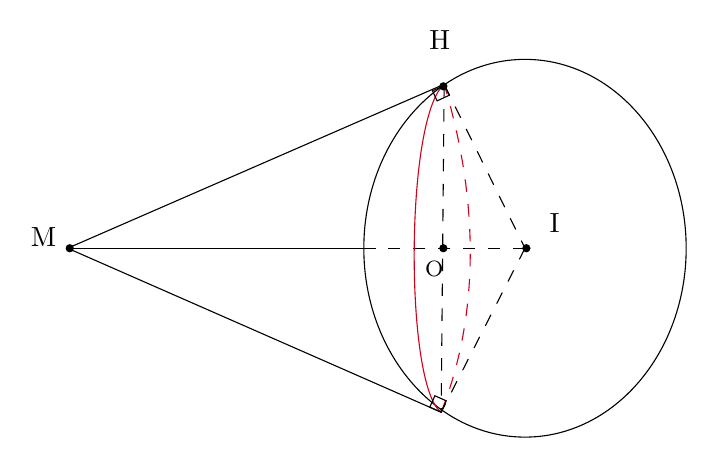
\begin{tikzpicture}[x=0.75pt,y=0.75pt,yscale=-1,xscale=1]
			%uncomment if require: \path (0,300); %set diagram left start at 0, and has height of 300
			%Shape: Ellipse [id:dp8222414503724227] 
			\draw   (334.68,147) .. controls (334.68,96.74) and (369.45,56) .. (412.34,56) .. controls (455.23,56) and (490,96.74) .. (490,147) .. controls (490,197.26) and (455.23,238) .. (412.34,238) .. controls (369.45,238) and (334.68,197.26) .. (334.68,147) -- cycle ;
			%Straight Lines [id:da5686780759798307] 
			\draw  [dash pattern={on 4.5pt off 4.5pt}]  (412.34,147) -- (334.68,147) ;
			%Straight Lines [id:da5121781501182883] 
			\draw    (334.68,147) -- (192,147) ;
			%Straight Lines [id:da5357941012794942] 
			\draw    (373.39,68) -- (192,147) ;
			%Straight Lines [id:da9685949970869305] 
			\draw    (371.95,226) -- (192,147) ;
			%Straight Lines [id:da7681419353872441] 
			\draw  [dash pattern={on 4.5pt off 4.5pt}]  (412.34,147) -- (371.95,226) ;
			%Straight Lines [id:da5806916153499093] 
			\draw  [dash pattern={on 4.5pt off 4.5pt}]  (373.39,68) -- (412.34,147) ;
			%Curve Lines [id:da817264284113064] 
			\draw [color={rgb, 255:red, 208; green, 2; blue, 27 }  ,draw opacity=1 ]   (373.39,68) .. controls (354.38,84.43) and (354.38,213.43) .. (371.95,226) ;
			%Straight Lines [id:da9825030542435118] 
			\draw  [dash pattern={on 4.5pt off 4.5pt}]  (373.39,68) -- (371.95,226) ;
			%Curve Lines [id:da9470182211565492] 
			\draw [color={rgb, 255:red, 208; green, 2; blue, 27 }  ,draw opacity=1 ] [dash pattern={on 4.5pt off 4.5pt}]  (371.95,226) .. controls (390.38,179.43) and (390.38,124.43) .. (373.39,68) ;
			%Shape: Free Drawing [id:dp4316645676344397] 
			\draw  [line width=3] [line join = round][line cap = round] (193,147) .. controls (193,147) and (193,147) .. (193,147) ;
			%Shape: Free Drawing [id:dp8882945718838733] 
			\draw  [line width=3] [line join = round][line cap = round] (373,69) .. controls (373,69) and (373,69) .. (373,69) ;
			%Shape: Free Drawing [id:dp630109668425459] 
			\draw  [line width=3] [line join = round][line cap = round] (373,147) .. controls (373,147) and (373,147) .. (373,147) ;
			%Shape: Free Drawing [id:dp9926156478969348] 
			\draw  [line width=3] [line join = round][line cap = round] (413,147) .. controls (413,147) and (413,147) .. (413,147) ;
			%Shape: Rectangle [id:dp10747987487669075] 
			\draw   (367.76,71.18) -- (373.61,68.47) -- (375.84,73.29) -- (370,76) -- cycle ;
			%Shape: Square [id:dp027493706007335694] 
			\draw   (368.92,218.07) -- (374.4,220.52) -- (371.95,226) -- (366.47,223.55) -- cycle ;
			% Text Node
			\draw (173,136) node [anchor=north west][inner sep=0.75pt]   [align=left] {M};
			% Text Node
			\draw (365,41) node [anchor=north west][inner sep=0.75pt]   [align=left] {H};
			% Text Node
			\draw (363,152) node [anchor=north west][inner sep=0.75pt]  [font=\footnotesize] [align=left] {O};
			% Text Node
			\draw (423,129) node [anchor=north west][inner sep=0.75pt]   [align=left] {I};
		\end{tikzpicture}
		\end{center}
		Mặt cầu $(S)$ có tâm $I(1;1;0)$ và bán kính $R=2$. Ta có: $\overrightarrow{IM}=(1;2;1)$ và $IM=\sqrt{6}$.\\
		Gọi $H$ là một tiếp điểm tùy ý khi kẻ tiếp tuyến từ $Oxyz$ đến mặt cầu, khi đó:\\ $MH=\sqrt{IM^2-R^2}=\sqrt{2}$.\\
		Gọi $O$ là tâm của đường tròn $(C)$ khi đó $IM \bot HO$ và $HO=r$.\\
		Ta có $HI.HM=HO.IM\Rightarrow r=\dfrac{HI.HM}{IM}=\dfrac{2\sqrt2}{\sqrt{6}}=\dfrac{2\sqrt{3}}{3}$.
		}
\end{ex}

\Closesolutionfile{ans}
\indapan{6}{ans/ans-0-B15}

\cauds%Câu đúng sai
\Opensolutionfile{ans}[ans/ans-0-B15-DS]

\begin{ex}%[2D1H4-3]Câu 1
	Cho hai phương trình mặt cầu $(C_1) \colon (x-2)^2+(y+2)^2+z^2=4$ và $(C_2) \colon x^2+y^2+z^2-2x+2y+4z-1=0$. Gọi $I_1, R_1$ là tâm và bán kính của $(C_1)$ và $I_2, R_2$ là tâm và bán kính của $(C_2)$. Hãy trả lời các ý sau:
	\choiceTF
	{Phương trình mặt cầu $(C_1), (C_2)$ có tọa độ tâm lần lượt là $I_1(2;-2;1)$ và $I_2(1;-1;-2)$}
	{\True Mặt cầu $(C_1)$ tiếp xúc với trục $Ox$ và $Oy$}
	{Khoảng cách nhỏ nhất của điểm $I_1$ đến mặt cầu $(C_2)$ có độ lớn bằng $1$}
	{\True $(C_1), (C_2)$ có một phương trình đường tròn giao tuyến là: $2x-2y+4z+3=0$}
	\loigiai{
	\begin{itemchoice}
		\itemch Sai. Vì $(C_1) \colon \heva{&\text{Tâm } I_1(2;-2;0)\\&R_1=2}$ và $(C_2) \colon \heva{&\text{Tâm } I_2(1;-1;-2)\\&R_2=\sqrt{7}}$.
		\itemch Đúng. Vì $d(I_1;Ox)=\dfrac{\left| \vec{i} \wedge \vec{OI_1} \right|}{\left| \vec{i} \right|}=2=R$ và $d(I_1;Oy)=\dfrac{\left| \vec{j} \wedge \vec{OI_1} \right|}{\left| \vec{j} \right|}=2=R$.
		\itemch Sai. Vì $I_2I_1=\sqrt{1^2+(-1)^2+2^2}=\sqrt{6}$, nhận xét $I_2I_1<R_1+R_2 \Leftrightarrow I_2I_1<2+\sqrt{7}$. Vậy khoảng cách nhỏ nhất của điểm $I_1$ đến mặt cầu $(C_2)$ có công thức:\\
		$d(I_1;(C_2))_{min}=\left| I_2I_1-R_2 \right|=\sqrt{7}-\sqrt{6}$.
		\itemch Đúng. Vì $\heva{&(x-2)^2+(y+2)^2+z^2=4 \\&x^2+y^2+z^2-2x+2y+4z-1=0} \Leftrightarrow \heva{&x^2+y^2+z^2-4x+4y-4=0 (1) \\&x^2+y^2+z^2-2x+2y+4z-1=0 (2)}$.\\
		Lấy $(1)-(2) \Rightarrow -2x+2y-4z-3=0 \Leftrightarrow 2x-2y+4z+3=0$.
	\end{itemchoice}
	}
\end{ex}

\begin{ex}%[2D1H4-3]Câu 2
	Trong không gian $Oxyz$, mặt cầu $(S)$ có tâm $I(1;0;-1)$ và có bán kính $R=\sqrt{2}$.
	\choiceTF
	{Phương trình của $(S)$ là $(x-1)^2+y^2+(z+1)^2=\sqrt{2}$}
	{Mặt cầu $(S)$ đi qua điểm  $I(1;0;-1)$}
	{\True Điểm $A(2;2;2)$ nằm ngoài phương trình mặt cầu $(S)$}
	{\True Các điểm nằm trên mặt cầu $(S)$ cách tâm $I$ một khoảng bằng $\sqrt{2}$}
	\loigiai{
		Theo đề bài ta có $\heva{&I(1;0;-1)\\&R=\sqrt{2}} \Rightarrow (S) \colon (x-1)^2+y^2+(z+1)^2=2$
		\begin{itemchoice}
			\itemch Sai.
			\itemch Sai. Vì $(1-1)^2+0^2+(-1+1)^2=0 \ne 2$.
			\itemch Đúng. Vì $(2-1)^2+2^2+(2+1)^2=14>2$.
			\itemch Đúng. Vì khoảng cách từ các điểm nằm trên mặt cầu $(S)$ cách tâm $I$ bằng bán kính $R=\sqrt{2}$.
		\end{itemchoice}
	}
\end{ex}

\begin{ex}%[2D1H4-3]Câu 3
	Trong không gian với hệ trục tọa độ $Oxyz$, cho có phương trình $(C) \colon x^2+y^2+z^2+2(m+2)x-2(m-3)z+m^2-1=0$
	\choiceTF
	{\True Phương trình $(C)$ luôn là phương trình mặt cầu}
	{Phương trình mặt cầu $(C)$ luôn có tâm $I(-m-2;m-3;-m^2-1)$ với $m \in \mathbb{R}$}
	{\True Với $m=1$ thì phương trình $(C)$ là mặt cầu có bán kính nhỏ nhất}
	{Phương trình mặt cầu $(C)$ luôn đi qua gốc tọa độ}
	\loigiai{
		\begin{itemchoice}
			\itemch Đúng. Vì $(C)$ là phương trình mặt cầu dạng tổng quát với các hệ số:\\
			$a=-(m+2),b=0,c=m-3,d=m^2-1 \Rightarrow$ Để $(C)$ là phương trình mặt cầu: $a^2+b^2+c^2-d>0$\\
			$\Leftrightarrow (m+2)^2+(m-3)^2-(m^2-1)>0 \Leftrightarrow m^2-2m+14>0$ (luôn đúng).
			\itemch Sai. Vì tâm $I(a;b;c) \Leftrightarrow I(-m-2;0;m-3)$
			\itemch Đúng. Vì $R=\sqrt{a^2+b^2+c^2-d}=\sqrt{m^2-2m+14}=\sqrt{(m-1)^2+13} \ge \sqrt{13}$.\\
			Dấu $"="$ xảy ra khi và chỉ khi $m-1=0 \Leftrightarrow m=1$.
			\itemch Sai. Vì thay $x=0,\,y=0,\,z=0$ vào $(1)$ ta có:\\
			$0^2+0^2+0^2+2(m+2).0-2(m-3).0+m^2-1=0 \Leftrightarrow m^2-1=0 \Leftrightarrow  m=\pm 1$.\\
			Nên phương trình $(1)$ là mặt cầu luôn đi qua gốc tọa độ chỉ khi $m=\pm 1$
		\end{itemchoice}
	}
\end{ex}

\begin{ex}%[2D1H4-3]Câu 4
	Trong không gian $Oxyz$, Cho $A(2;1;1)$, $B(1;1;-3)$ và mặt cầu $(S)$ có tâm $I(1;-3;-1)$ bán kính $R=2$.
	\choiceTF
	{\True Phương trình mặt cầu $(S)$ có phương trình $(x-1)^2+(y+3)^2+(z+1)^2=4$}
	{\True Hai điểm $A,\,B$ đều nằm ngoài mặt cầu $(S)$}
	{\True Khoảng cách từ tâm $I$ đến trung điểm của đoạn thẳng $AB$ có độ lớn bằng $\dfrac{\sqrt{65}}{2}$}
	{Phương trình mặt cầu tâm $A$ có đường kính bằng $4$ có mặt phẳng giao tuyến với mặt cầu $(S)$ có phương trình là: $x+4y+2z-3=0$}
	\loigiai{
		\begin{itemchoice}
			\itemch Đúng. Vì phương trình $(S)$ có phương trình: $(x-1)^2+(y+3)^2+(z+1)^2=4$.
			\itemch Đúng. Vì ta thay lần lượt hai điểm $A(2;1;1)$ và $B(1;1;-3)$ vào $(S)$:\\ $\heva{&(2-1)^2+(1+3)^2+(1+1)^2=21>4\\&(1-1)^2+(1+3)^2+(-3+1)^2=20>4}$
			\itemch Đúng. Gọi $M$ là trung điểm $AB \Rightarrow M\left(\dfrac{3}{2};1;-1\right)$\\
			$\Rightarrow IM=\sqrt{\left(\dfrac{3}{2}-1\right)^2+(1-(-3))^2+(-1-(-1))^2}=\dfrac{\sqrt{65}}{2}$.
			\itemch Sai. Gọi $(S_1)$ là phương trình mặt cầu tâm $A(2;1;1)$ và bán kính $R_1=2$ có phương trình:\\
			$(S_1) \colon (x-2)^2+(y-1)^2+(z-1)^2=4$\\
			Ta có: $\heva{&(S) \colon (x-1)^2+(y+3)^2+(z+1)^2=4 \,(1)\\&(S_1) \colon (x-2)^2+(y-1)^2+(z-1)^2=4 \,(2)}$\\
			Lấy $(1)-(2)$ ta có: $2x+8y+2z+5=0$
		\end{itemchoice}
	}
\end{ex}

\Closesolutionfile{ans}
\indapan{3}{ans/ans-0-B15-DS}

\Opensolutionfile{ans}[ans/ans-0-B15-KQ]
\caukq%Câu kết quả

\begin{ex}%[2D1N4-1]Câu 1
	Trong không gian với hệ trục tọa độ $Oxyz$, cho các phương trình sau:\\
	$(x-2)^2+(y+3)^2+z^2=5 \,(1)$\\
	$x^2+y^2+z^2-2x+4y-6z+1=0 \,(2)$\\
	$3x^2+3y^2+3z^2-6x+3y+21=0 \,(3)$\\
	Có tất cả bao nhiêu phương trình là phương trình mặt cầu
	\shortans{$2$}
	\loigiai{
	$\bullet (1)$ là phương trình mặt cầu dạng chính tắc.\\
	$\bullet (2)$ là phương trình mặt cầu do các hệ số $a=1,b=-2,c=3,d=1$ thỏa mãn $a^2+b^2+c^2-d>0 \Rightarrow 13>0$.\\
	$\bullet (3)$ không là phương trình mặt cầu do các hệ số $a=1,b=-\dfrac{1}{2},c=0,d=7$ không thỏa mãn $a^2+b^2+c^2-d>0 \Rightarrow -\dfrac{23}{4}>0$(Sai).}
\end{ex}

\begin{ex}%[2D1N4-1]Câu 2
	Trong không gian với hệ trục tọa độ $Oxyz$, Biết các giá trị $m$ thỏa mãn đồng thời các phương trình sau là phương trình mặt cầu có dạng $m<\dfrac{a}{b}$ và $m>c$.\\
	a) $x^2+y^2+z^2-2mx+2(m+1)y-4z+1=0$.\\
	b) $x^2+y^2+z^2-2(m-3)x-4mz+8=0$.\\
	Tinh tổng $G=5a-b-c$
	\shortans{$-1$}
	\loigiai{
	a) Phương trình có các hệ số $a=m,\,b=-(m+1),\,c=2,\,d=1.$\\
	Điều kiện: $a^2+b^2+c^2-d>0\Leftrightarrow m^2+(m+1)^2+2^2-1>0\Leftrightarrow 2m^2+2m+4>0\Leftrightarrow m\in \mathbb{R}.$\\
	b) Phương trình có các hệ số $a=m-3,\,b=0,\,c=2m,\,d=8.$\\
	Điều kiện: $a^2+b^2+c^2-d>0\Leftrightarrow (m-3)^2+(2m)^2-8>0\Leftrightarrow 5m^2-6m+1>0\Leftrightarrow \hoac{&m<\dfrac{1}{5}\\&m>1}$
	Vậy $m=1,\,n=5,\,p=1 \Rightarrow G=-1$.
	}
\end{ex}

\begin{ex}%[2D1N4-1]Câu 3
	Trong không gian với hệ trục tọa độ $Oxyz$, cho mặt cầu $(S)$ có phương trình $x^2+y^2+z^2+4x-2y-4=0$. Tính bán kính $R$ của $(S)$.
	\shortans{$3$}
	\loigiai{
	Ta có: $a=-2,b=1,c=0,d=-4\Rightarrow $ Bán kính $R=\sqrt{a^2+b^2+c^2-d=3}$
	.}
\end{ex}

\begin{ex}%[2D1N4-1]Câu 4
	Trong không gian với hệ trục tọa độ $Oxyz$, có tất cả bao nhiêu giá trị nguyên $m$ để phương trình $x^2+y^2+z^2+4mx+2my-2mz+9m^2-28=0$ là phương trình mặt cầu?
	\shortans{$7$}
	\loigiai{
	Ta có $x^2+y^2+z^2+4mx+2my-2mz+9m^2-28=0$\\
	$\Leftrightarrow (x+2m)^2+(y+m)^2+(z-m)^2=28-3m^2 \,(1)$.\\	$(1)$  là phương trình mặt cầu $\Leftrightarrow 28-3m^2>0\Leftrightarrow -\sqrt{\dfrac{28}{3}}<m<\sqrt{\dfrac{28}{3}}$.\\
	Do $m$ nguyên nên $m\in \left\lbrace -3;-2;-1;0;1;2;3 \right\rbrace$.\\
	Vậy có $7$ giá trị của $m$ thỏa mãn yêu cầu bài toán.}
\end{ex}

\begin{ex}%[2D1N4-1]Câu 5
	Trong không gian với hệ trục tọa độ $Oxyz$, xét mặt cầu $(S)$ có phương trình dạng $x^2+y^2+z^2-4x+2y-2az+10a=0$. Tìm các giá trị thực của $a$ để $(S)$ có chu vi đường tròn lớn bằng $8\pi $.
	\shortans{$2$}
	\loigiai{
	Đường tròn lớn có chu vi bằng $8\pi $ nên bán kính của $(S)$ là $\dfrac{8\pi}{2\pi }=4$.\\
	Từ phương trình của $(S)$ suy ra bán kính của $(S)$ là $\sqrt{2^2+1^2+a^2-10a}$.\\
	Do đó: $\sqrt{2^2+1^2+a^2-10a}=4\Leftrightarrow \hoac{&a=-1\\&a=11}$
	.}
\end{ex}

\begin{ex}%[2D1N4-1]Câu 6
	Đầu in phun của một máy in 3D đang in bề mặt của một mặt cầu có phương trình: 
	$x^2+y^2+z^2+\dfrac{1}{5}x-\dfrac{1}{10}y+2z+\dfrac{1}{20}=0$. Tính khoảng cách từ đầu in phun đến tâm mặt cầu.
	\shortans{$0{,}98$}
	\loigiai{
	Mặt cầu có:\\
	Tâm $I\left(-\dfrac{1}{10};\dfrac{1}{20};-1\right)$ và bán kính $R=\sqrt{\left(-\dfrac{1}{10}\right)^2+\left(\dfrac{1}{20}\right)^2+(-1)^2-\dfrac{1}{20}}=\dfrac{\sqrt{385}}{20}$.\\
	Khoảng cách từ đầu in phun đến tâm mặt cầu chính bằng bán kính của mặt cầu:\\ $R=\dfrac{\sqrt{385}}{20}$
	.}
\end{ex}

\Closesolutionfile{ans}
\indapan{6}{ans/ans-0-B15-KQ}